\documentclass[xcolor=pdftex,dvipsnames,table,mathserif,aspectratio=169]{beamer}
\usetheme{metropolis}
%\usetheme{Darmstadt}
%\usepackage{times}
%\usefonttheme{structurebold}

\usepackage[english]{babel}
%\usepackage[table]{xcolor}
\usepackage{pgf,pgfarrows,pgfnodes,pgfautomata,pgfheaps}
\usepackage{amsmath,amssymb,setspace}
\usepackage[latin1]{inputenc}
\usepackage[T1]{fontenc}
\usepackage{relsize}
\usepackage[absolute,overlay]{textpos} 
\newenvironment{reference}[2]{% 
  \begin{textblock*}{\textwidth}(#1,#2) 
      \footnotesize\it\bgroup\color{red!50!black}}{\egroup\end{textblock*}} 

\DeclareMathSizes{10}{10}{6}{6} 


\title [Dynamic Oligopoly I]{Switching Costs}
\author{C.Conlon }
\institute{Grad IO }
\date{Fall 2019}
\setbeamerfont{equation}{size=\tiny}
\begin{document}

\begin{frame}
\titlepage
\end{frame}



\begin{frame}{State Dependence}
Think about a static model like BLP
\begin{eqnarray*}
u_{ijt} = \beta_i x_{jt} - \alpha_i p_{jt} + \xi_{jt} + \varepsilon_{ijt}
\end{eqnarray*}
\begin{itemize}
\item Suppose I have panel data on consumer $i$'s purchases and I observe that the consumer chooses different brands over time
\item Why do you switch brands?  $\beta_i$ are persistent.
\begin{enumerate}
\item New $\varepsilon \rightarrow$ not helpful!
\item Price responses $\rightarrow$ may wrongly attribute all effects to price.
\item $\xi_{jt}$ not correlated across individuals but may include things like advertising, etc.
\end{enumerate}
\item Challenge is explaining both \alert{persistence} and \alert{switching} behavior.
\end{itemize}
\end{frame} 



\begin{frame}{Terminology}
Sometimes we call these models \alert{switching costs} and other times \alert{state dependence}
\begin{eqnarray*}
u_{ijt} = \beta_i x_{jt} - \alpha_i p_{jt} + \xi_{jt} + \alert{\gamma_i \cdot I[y_{i,t-1}=j]} + \varepsilon_{ijt} 
\end{eqnarray*}
\begin{itemize}
\item The idea is purchases in period $t-1$ have a causal effect on utility in period $t$
\item We can think of this as either increasing utility for $j$ if you previously purchased it or providing an additional cost if $y_{it} \neq y_{i,t-1}$.
\end{itemize}
\end{frame} 


\begin{frame}{Why Do We Care?}
\begin{itemize}
\item Switching costs appear to be a real friction in the economy.
\item Consumers are often highly persistent in product choices.
\begin{itemize}
\item Because they really like the product?
\item Because they are unaware of alternatives?
\item Because they are lazy?
\end{itemize}
\item Extremely important in the market for \alert{health insurance}. Consumers in ACA (Obamacare) exchanges would have saved \$610/yr on average if they switched to a lower cost plan in the same tier.
\begin{itemize}
\item Real costs associated with switching: checking to see if my doctor takes the other insurer, calculating expected expenditures, etc.
\end{itemize}
\item Can we reduce or exploit frictions with laws? defaults? etc.
\end{itemize}
\end{frame} 

\begin{frame}{Why Do We Care?}
\begin{itemize}
\item Switching costs are another way to escape the Bertrand trap for firms which sell relatively undifferentiated products.
\item Old idea going back to Klemperer (1995), Farrell and Klemperer (2007). Do switching costs make markets more or less competitive?
\item Two incentives:
\begin{itemize}
\item \alert{Investment}: Sign up a bunch of consumers today and they will be ``sticky'' to you in the future $\rightarrow$ \alert{lower prices}
\item \alert{Harvesting}: You have additional market power over your ``sticky'' customers $\rightarrow$ \alert{higher prices}
\end{itemize}
\item Most people believe that \alert{harvesting} dominates, and switching costs lead to \alert{higher} prices. (But not always...)
\end{itemize}
\end{frame} 

\begin{frame}{Cabral (JMR 2008)}
Consider dynamic optimization problem faced by firm $i$ with a vector of prices $\mathbf{p}$ and state variables (shares) $\mathbf{x}$ and switching costs $s$:
\begin{eqnarray*}
V_i(\mathbf{x},\mathbf{p},s) = (p_i - c_i) \cdot q_i(\mathbf{x},\mathbf{p},s) + \beta \tilde{V}_i(\mathbf{x},\mathbf{p},s)
\end{eqnarray*}
with FOC
\vspace{-.3cm}
\begin{eqnarray*}
q_i(\mathbf{x},\mathbf{p},s) +  (p_i - c_i) \cdot \underbrace{\frac{\partial q_i(\mathbf{x},\mathbf{p},s)}{\partial p_i}}_{q_i'} +  \beta  \underbrace{\frac{\partial \tilde{V}_i(\mathbf{x},\mathbf{p},s)}{\partial p_i}}_{\tilde{V}_i' \frac{\partial q_i}{\partial p_i}}
\end{eqnarray*}
\vspace{-.3cm}
Define $\tilde{V}_i' \equiv \frac{\partial \tilde{V}_i}{\partial q_i}$ (note w.r.t. $q_i$ not $p_i$). So that:
\begin{eqnarray*}
p_i - c_i = \underbrace{\frac{q_i}{-q_i'}}_{\alert{\mbox{Harvesting}}} - \underbrace{\beta \tilde{V}_i'}_{\alert{\mbox{Investment}}}
\end{eqnarray*}
\end{frame} 

\begin{frame}{Cabral (JMR 2008)}
\begin{eqnarray*}
p_i - c_i = \underbrace{\frac{q_i}{-q_i'}}_{\alert{\mbox{Harvesting}}} - \underbrace{\beta \tilde{V}_i'}_{\alert{\mbox{Investment}}}
\end{eqnarray*}
\vspace{-.3cm}
\begin{itemize}
\item Second term (dynamic benefit of increasing $q_i$ today) is ``investing'' in marketshare and leads to lower PCM.
\item First term is additional market power from switching costs and leads to higher PCM.
\item Take derivatives w.r.t. $s$.
\begin{itemize}
\item It is clear that $|q_i'|$ is decreasing in $s$. Higher switching costs increase static market power.
\item $q_i$ is ambiguous across firms. (So net effect is ambiguous across $i$).
\item $V_i'$ should be zero if $s=0$. And $V_i'$ is increasing in $s$. (Always positive).
\end{itemize}
\item Harvesting can be $\pm$, Investment always $-$.
\end{itemize}
\end{frame} 


\begin{frame}{How do we model these?}
\begin{eqnarray*}
u_{ijt} = \beta_i x_{jt} - \alpha_i p_{jt} + \xi_{jt} + \alert{\gamma_i \cdot I[y_{i,t-1}=j]} + \varepsilon_{ijt} 
\end{eqnarray*}
\begin{itemize}
\item We can include \alert{lagged choice} in utility of the agent. (First order Markov)
\item Could include two lagged choices if we wanted to.
\item Consumers are \alert{not} forward looking. Why?
\item Has some problems: endogeneity, correlation in $\epsilon_{ijt}$ over time, etc.
\item Fundamental question: How do we identify separately from persistent brand preference?
\item Dube, Histch, Rossi approach: Throw a ton of heterogeneity at the problem.
\end{itemize}
\end{frame} 

\begin{frame}{Mixture of Normals}
Let $\theta_i =[\alpha_i,\beta_i,\gamma_i]$.
\begin{itemize}
\item For each individual draw a class $k$ from a multinomial distribution $\pi$.
\item Now draw $\theta_i \sim MVN(\mu_k, \Sigma_k)$.
\item Idea is that $P(\theta_i | \pi,\mu,\Sigma) = \sum_k \pi_k \phi(\theta_i | \mu_k, \Sigma_k)$ is a mixture of normals. \pause
\item These models are highly flexible (around 4-5 normals tends to well approximate most distributions).
\item But hard to estimate! (Problem is highly non-convex, EM algorithm is slow).
\item In order to do MCMC estimation we have to assume some hyper-parameters $b$ so that we can put a prior on $\pi$ as well as $\mu_k,\Sigma_k$.
\end{itemize}
\end{frame} 



\begin{frame}{Switching Costs in Orange Juice}
\begin{center}
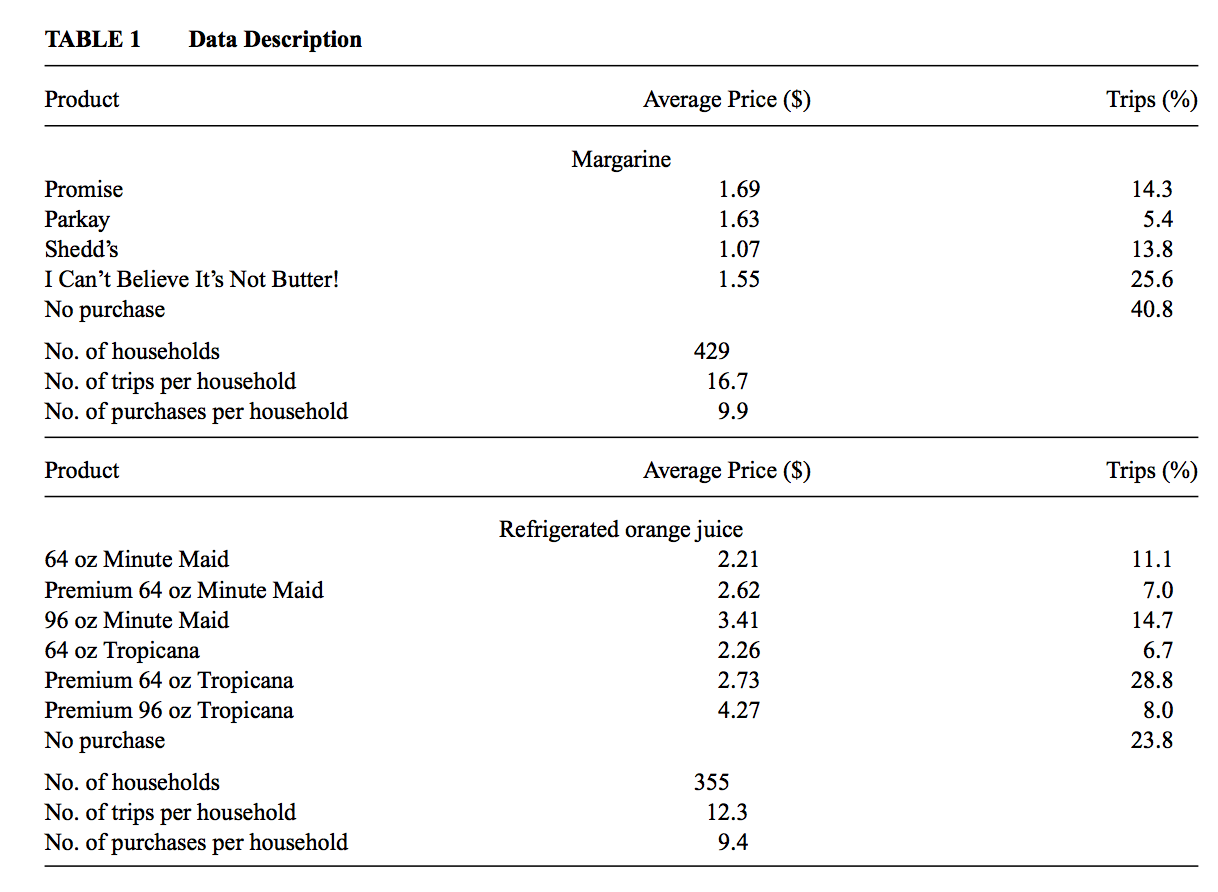
\includegraphics[scale=0.5]{resources/oj_t1.png}
\end{center}
\end{frame}

\begin{frame}{Switching Costs in Orange Juice}
\begin{center}
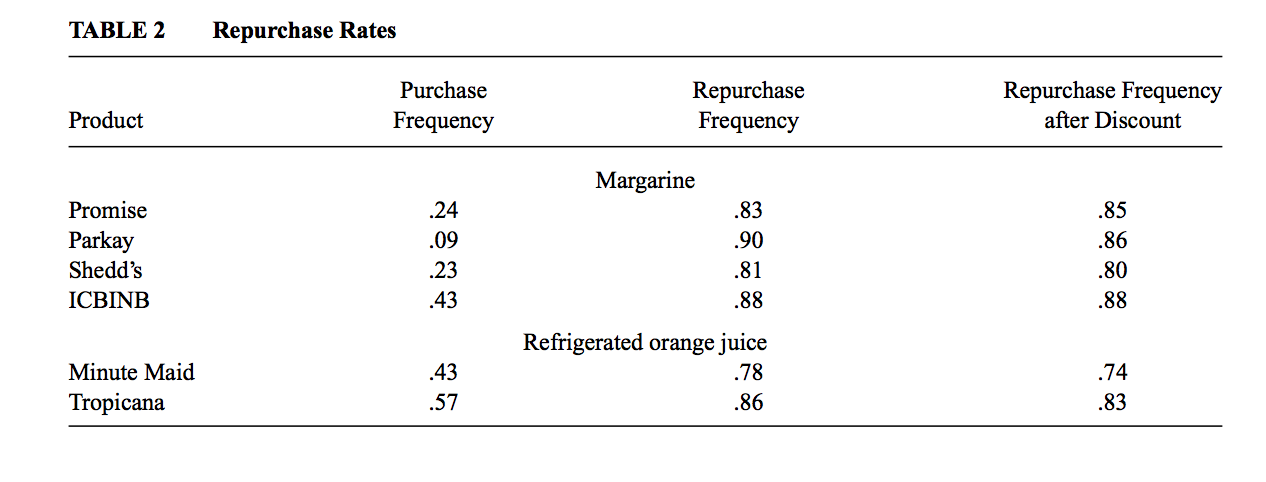
\includegraphics[scale=0.5]{resources/oj_t2.png}
\end{center}
\end{frame}

\begin{frame}{Switching Costs in Orange Juice}
\begin{center}
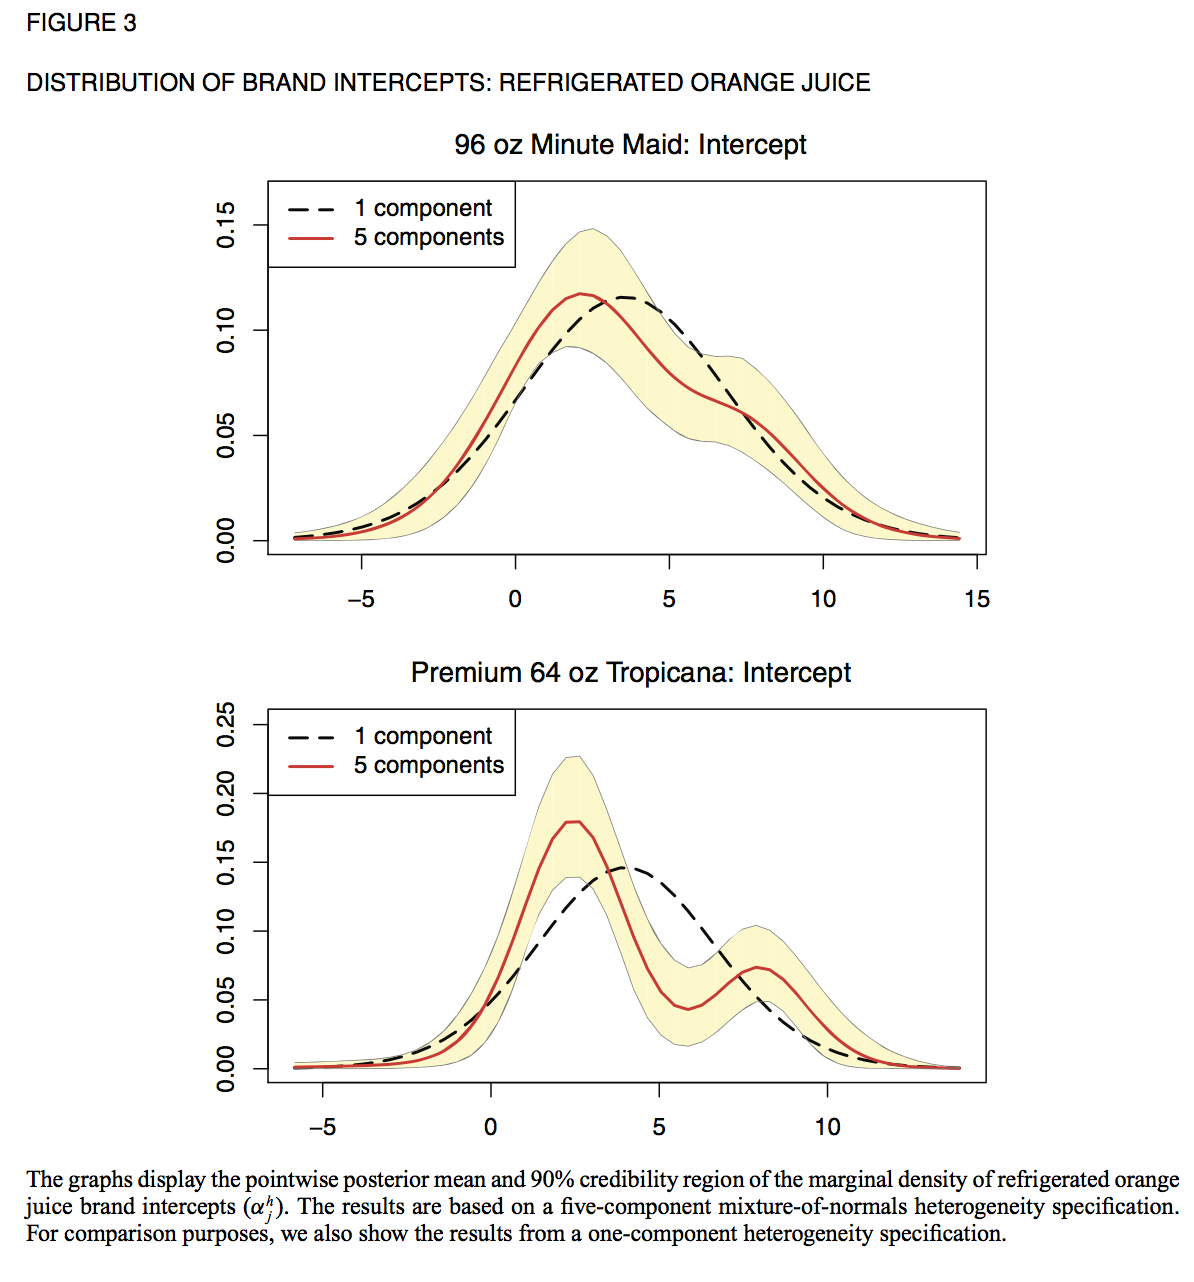
\includegraphics[scale=0.33]{resources/OJ_F3.png}
\end{center}
\end{frame}

\begin{frame}{Switching Costs in Orange Juice}
\begin{center}
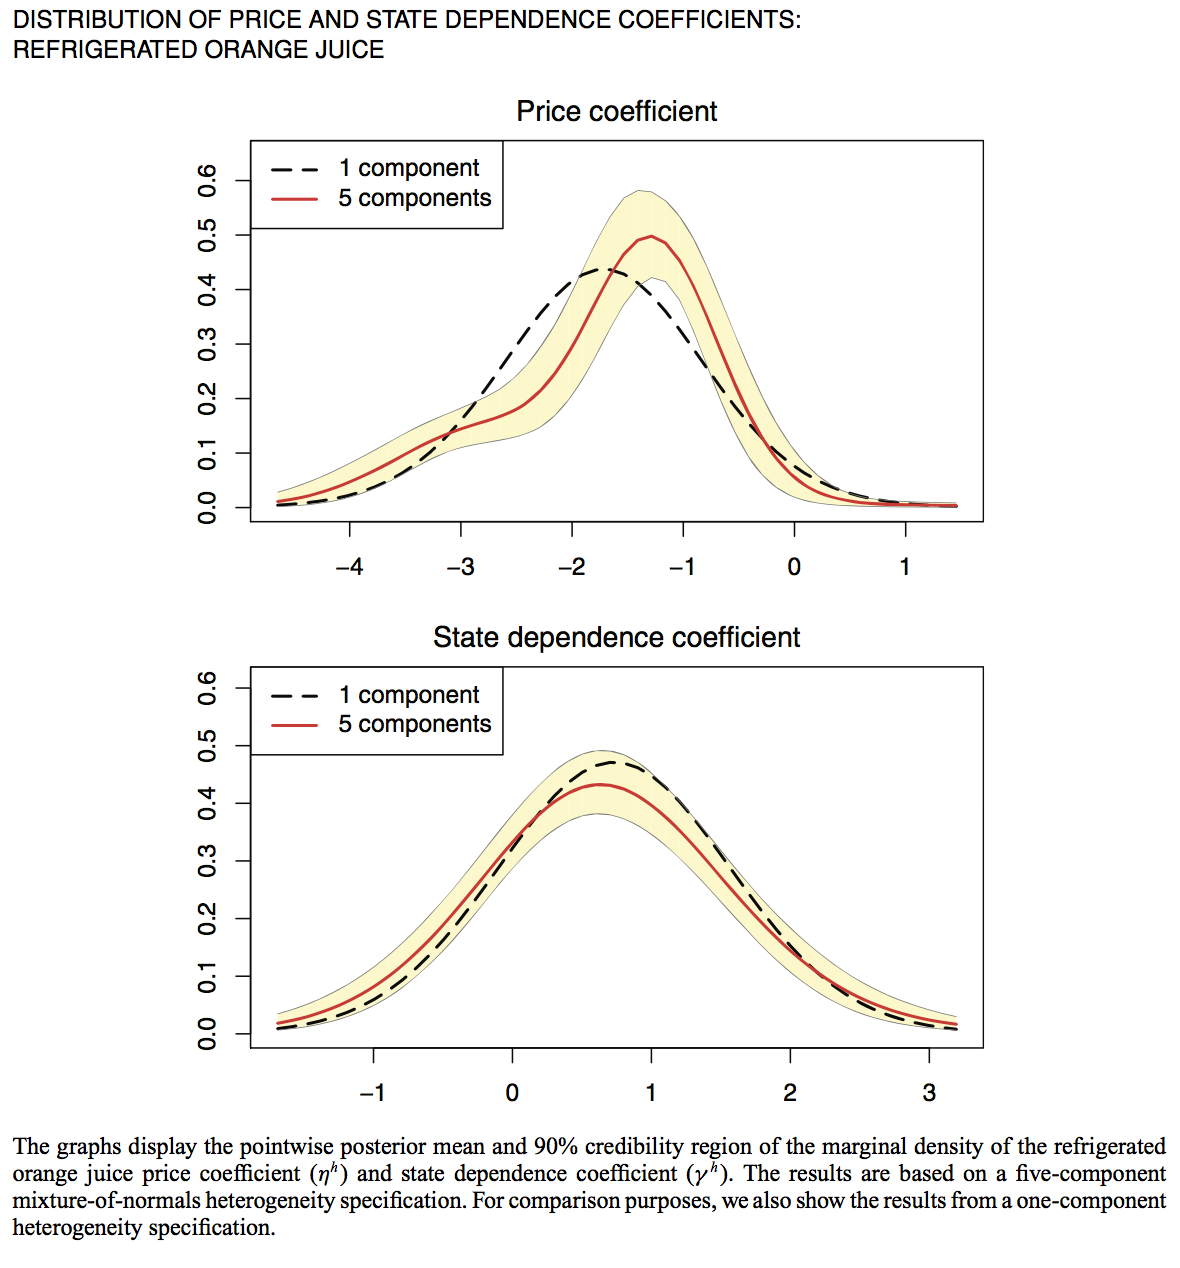
\includegraphics[scale=0.33]{resources/OJ_F4.png}
\end{center}
they also try 10 components...
\end{frame}

\begin{frame}{Identification}
\begin{itemize}
\item Lots of price changes in the category. Imagine two brands $(P,C)$ and each one can set two prices $\{H,L\}$.
\item We observe the sequence $D_1(H,H) = C, D_2(H,L) = C, D_3(H,H) = C, D_4(L,H) = P$.
\item If we see that $D_5(H,H/L) = P$ then we find evidence of state dependence.
\item Likewise we can see you switch, become sticky, and switch back later.
\end{itemize}
\end{frame} 

\begin{frame}{Identification/Robustness}
\begin{itemize}
\item The authors re-arrange the order of purchases within an individual and re-estimate.
\item If this was persistent heterogeneity they should still spuriously find a large $\gamma$
\item They do not!
\end{itemize}
\end{frame}
 
\begin{frame}{Switching Costs in Orange Juice}
\begin{center}
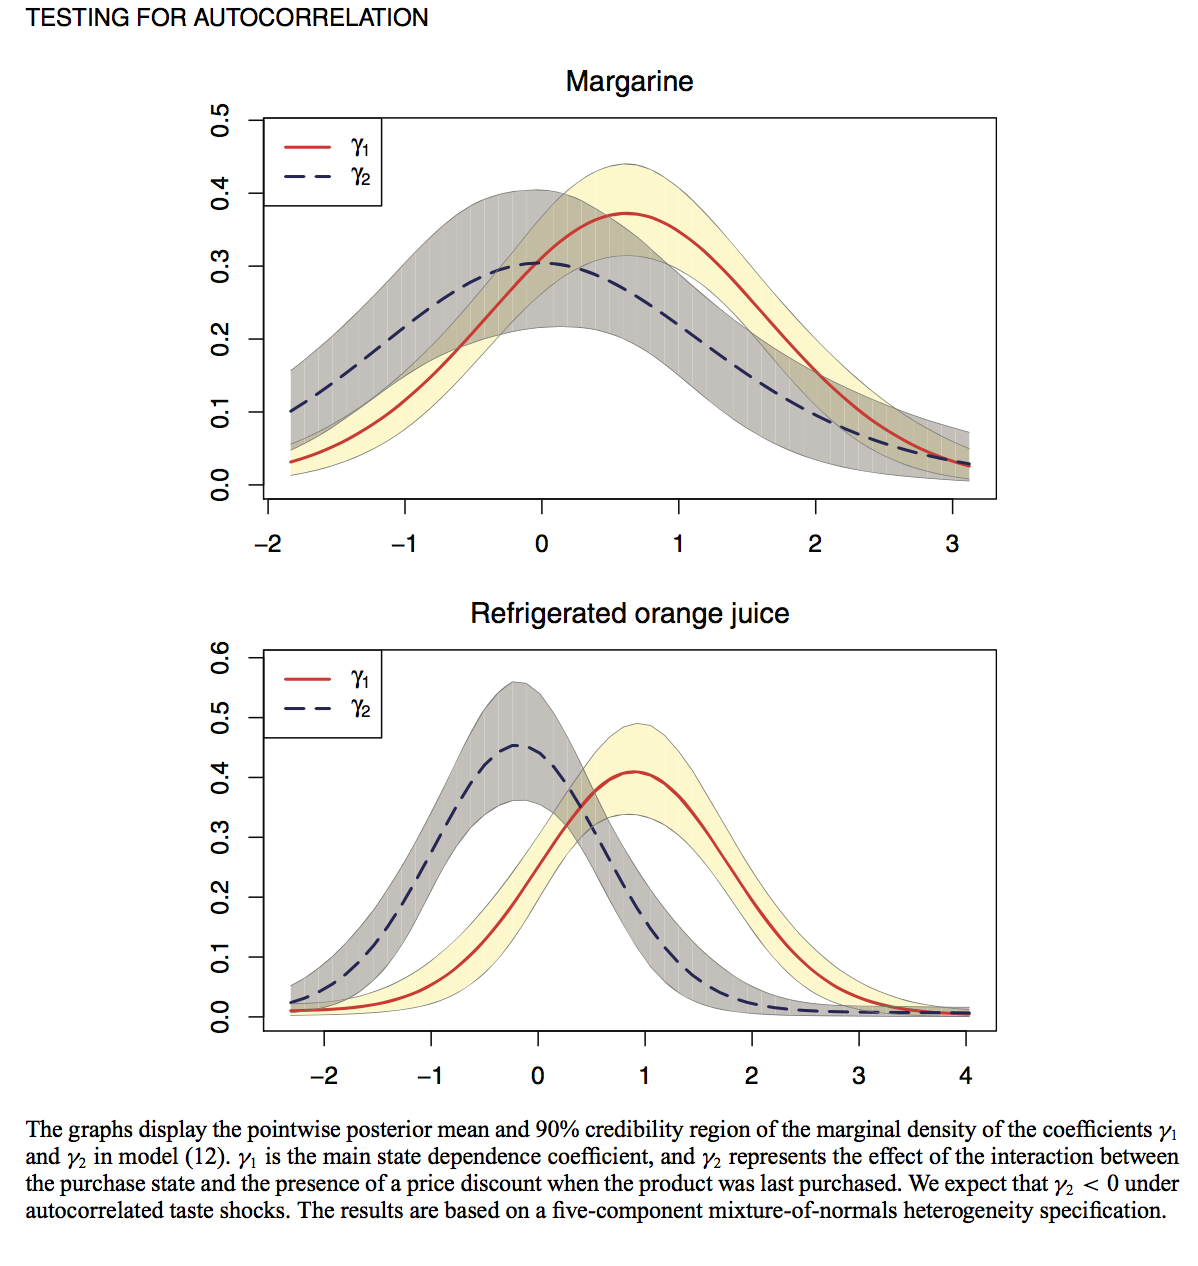
\includegraphics[scale=0.33]{resources/OJ_F5.png}
\end{center}
\end{frame}


\begin{frame}{Switching Costs in Orange Juice}
\begin{center}
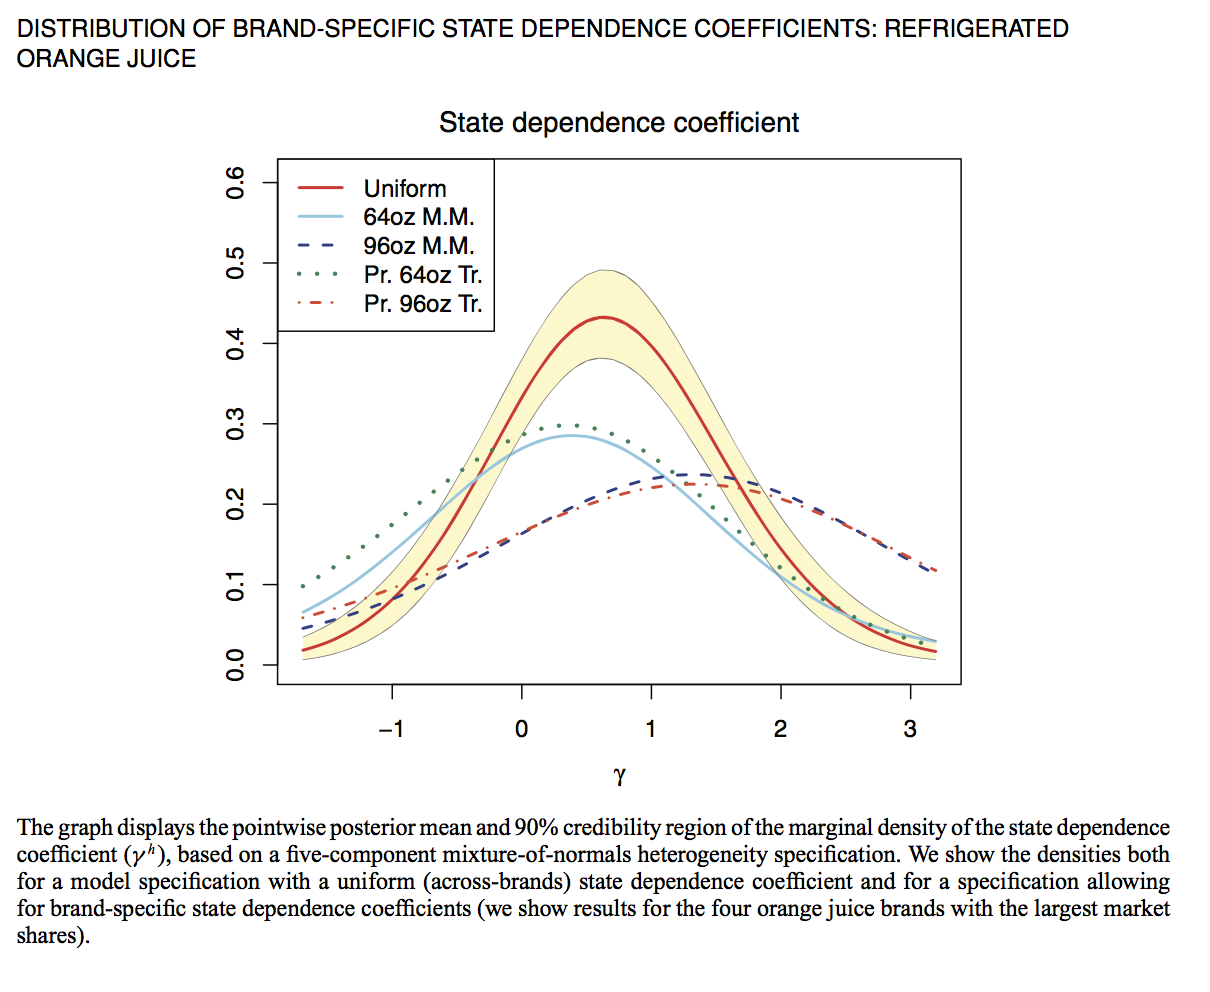
\includegraphics[scale=0.33]{resources/OJ_F8.png}
\end{center}
\end{frame}


\begin{frame}{Switching Costs in Orange Juice}
\begin{center}
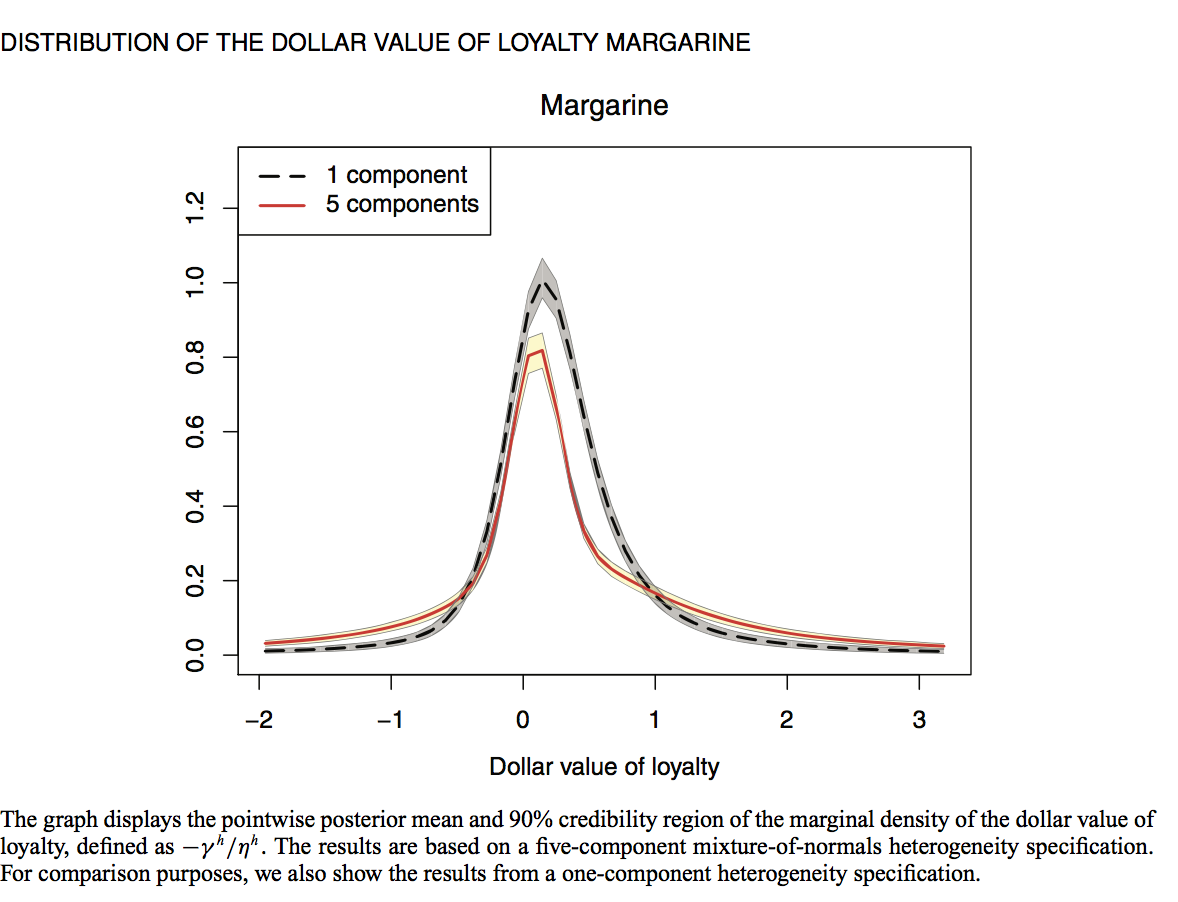
\includegraphics[scale=0.33]{resources/OJ_F11.png}
\end{center}
\end{frame}

\begin{frame}{Why Does this matter}
\begin{itemize}
\item Solve a dynamic programming problem like in Cabral (2008).
\item If we have just auto-correlation and no switching costs, there is NO harvesting incentive.
\item If we have switching costs than there is.
\item Very small switching costs can make markets MORE competitive.
\end{itemize}

\end{frame}


\begin{frame}{Switching Costs in Orange Juice}
\begin{center}
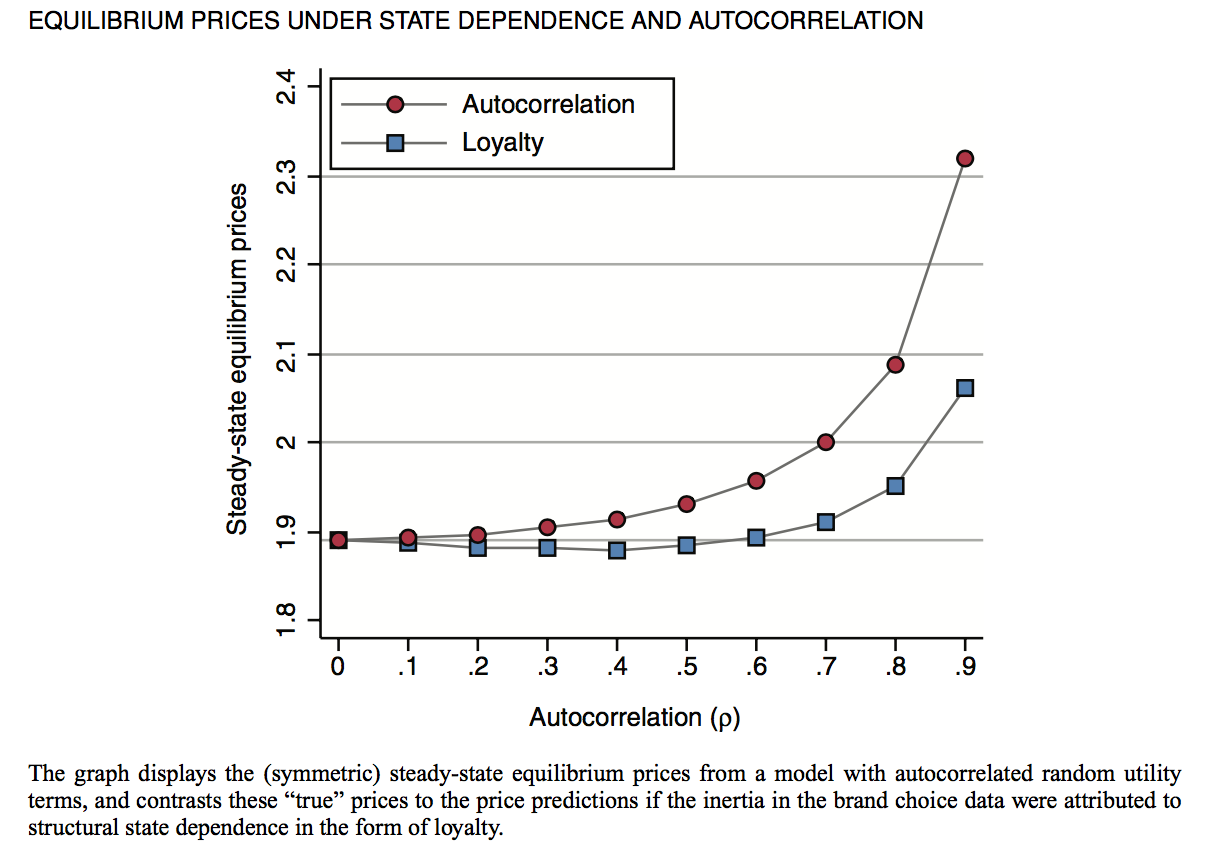
\includegraphics[scale=0.33]{resources/OJ_F12.png}
\end{center}
\end{frame}

\begin{frame}{What are Network Effects?}
\begin{itemize}
\item An important aspect of many digital markets today is \textit{network effects}.
\item Main idea is that you value the good more if other people use it.
\begin{itemize}
\item Social Networks: Facebook, Instagram, Twitter, Tindr, etc.
\item Statistical Packages: Stata, R, Matlab, etc.
\item P2P Platforms: Ebay, Etsy, Alibaba, Uber.
\item Software Platforms: iOS, Android, Windows.
\item Game Consoles: PS4, XBox One, etc.
\end{itemize}
\item This creates a \alert{lock in} effect.
\begin{itemize}
\item You may have an incentive to underprice initially to drive adoption.
\item There may be benefits to being early to market.
\item Markets can \alert{tip} one way or another.
\end{itemize}
\item Two-sided markets are another important issue (Developers, Developers, Developers!) 
\end{itemize}
\end{frame}


\begin{frame}{What are Network Effects?}
\begin{itemize}
\item Consumers make adoption decision that is durable (or irreversible) and depends on two things:
\begin{itemize}
\item The share of users on the same platform $\rho_{jt}$
\item Beliefs about the future of $E[\rho_{j,t}]$
\end{itemize}
\item Because beliefs are important, multiple equilibria can arise
\item How do we measure the size/impact of indirect network effects?
\item Constructing a counterfactual equilibria in a world without network-effects is hard to do in practice.
\end{itemize}
\end{frame}

\begin{frame}{What are Network Effects?}
\begin{center}
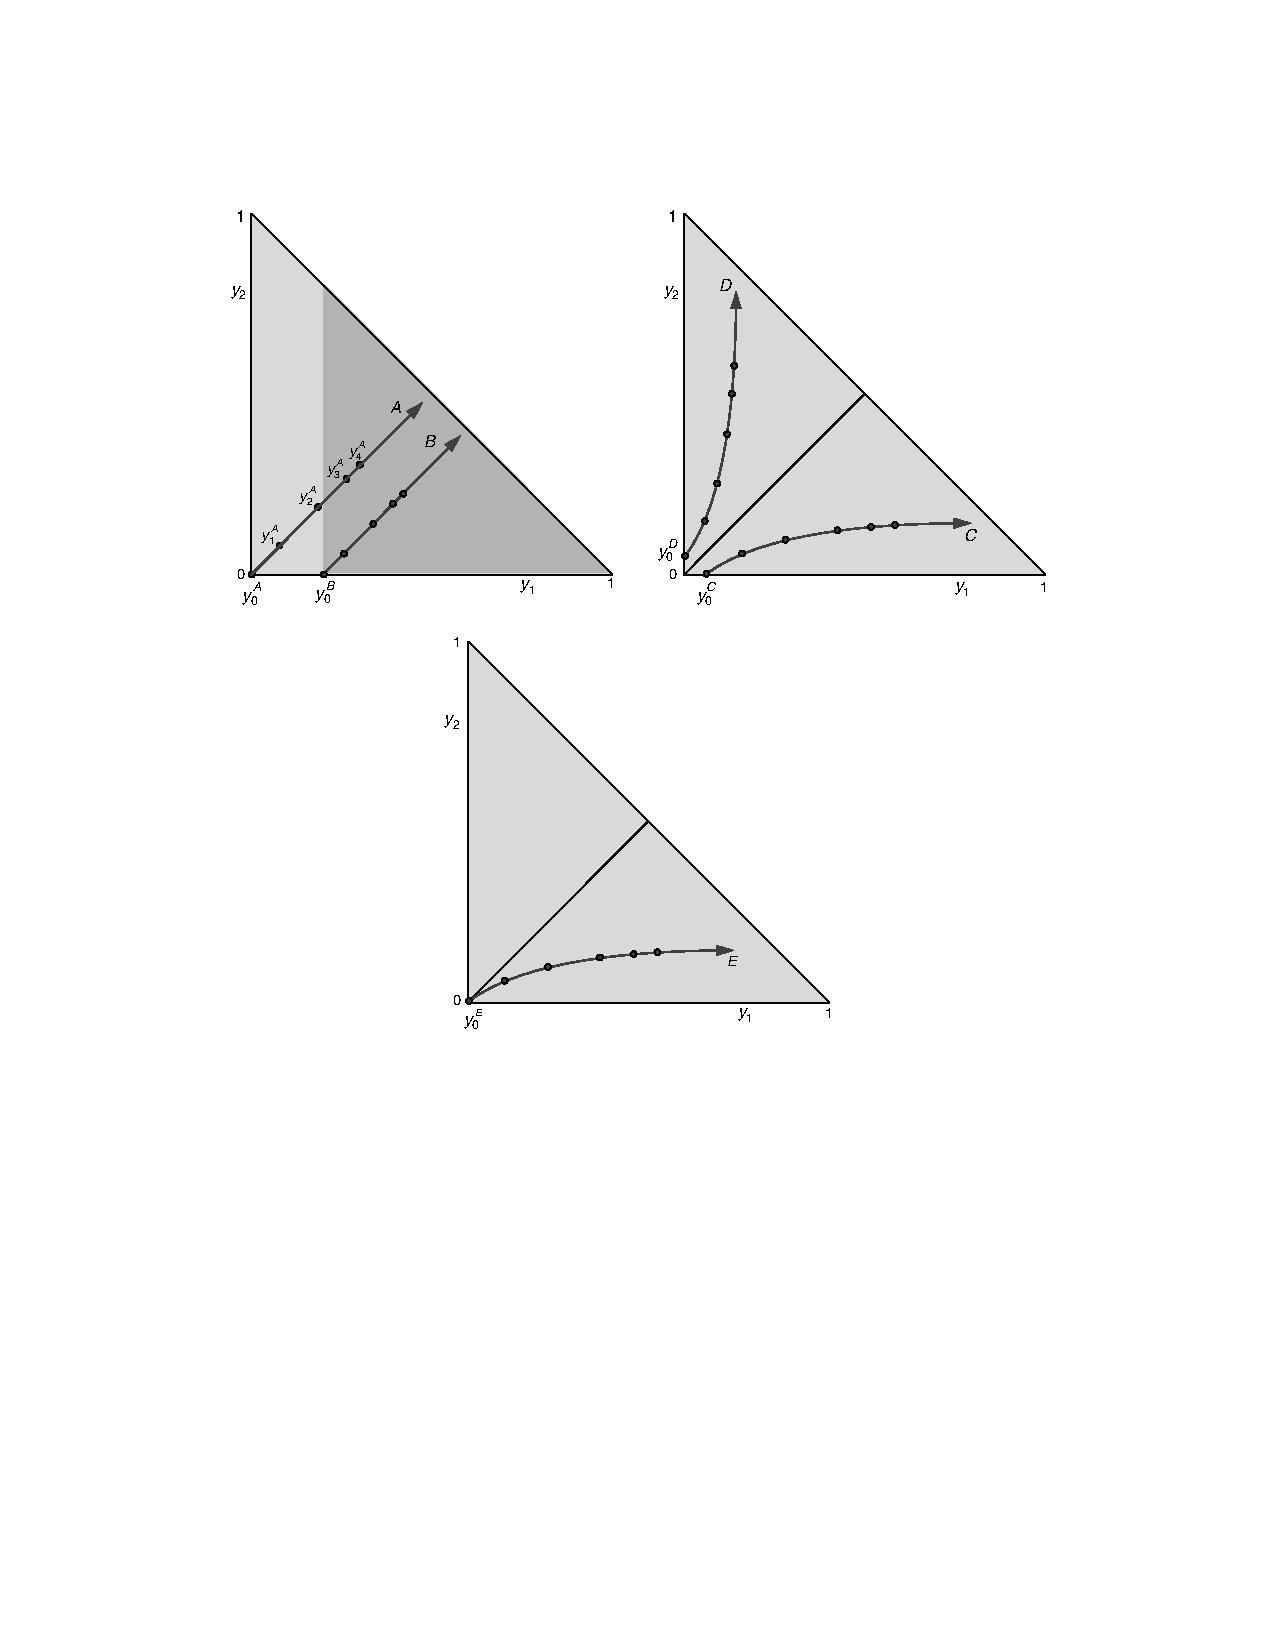
\includegraphics[scale=0.5]{resources/triangles.pdf}
\end{center}
\end{frame}


\begin{frame}{Dube, Hitsch, Chintagunta: Tipping}

\begin{itemize}
\item Start with two firms and $M=1$ mass of consumers
\item Installed base $y_{t} = [y_{1t},y_{2t}] \in [0,1]$ is the state space.
\item Assume that demand shock $\xi_{jt}~\sim \phi(\xi)$ is private information to the firm (similar to Seim's paper on video stores).
\item Timing of the game:
\begin{enumerate}
\item Firms learn $\xi_{jt}$ and set $p_{jt}$
\item Consumers adopt $\{1,2\}$ or delay purchase $=0$
\item Software firms supply a given number of titles $n_{jt}$
\item Sales are realized and firms receive profits. Consumers receive utility from $n_{jt}$ and in adoption period from platform itself.
\end{enumerate}
\item Information structure guarantees a unique best response (conjecture) and a pure-strategy equilibria.
\item Hence prices $p_{jt}$ contain a lot of information.
\end{itemize}
\end{frame}



\begin{frame}{}

\begin{itemize}
\item Titles depend on next period state variable: $n_{jt} = h_j(y_{j,t+1})$. Why?
\end{itemize}
\end{frame}

\begin{frame}{Consumers}
Need two things:
\begin{itemize}
\item Current prices and installed base $(p_t, y_t)$
\item Beliefs about the future $y_{t+1} = f^e(y_t,\xi_t)$ and conjecture about firm policy $p_{jt} = \sigma_j^e(y_t,\xi_t)$.
\end{itemize}
Utilities
\begin{itemize}
\item Flow from software: $u_j(y_{j,t+1}) = \gamma n_{jt} = \gamma h_j (y_{j,t+1})$
\item In PDV: $\omega_j (y_{t+1}) = E [ \sum_{k=0}^{\infty} \beta^k u_j(y_{j,t+1+k}) | y_{t+1}]$
\item This PDV trick is common (and helpful) and solves the recursion:
\begin{eqnarray*}
\omega_j(y_{t+1}) &=& u_j(y_{j,t+1}) + \beta \int  \omega_j( f^e(y_t,\xi_t)) \phi(\xi) \partial \xi\\
\end{eqnarray*}
\end{itemize}
\end{frame}

\begin{frame}{Consumers}
Choose $j$ to maximize choice specific value function (indirect utility) logit error :
\begin{eqnarray*}
v_j (y_t,\xi_t,p_t) &=& \delta_j + \omega_j( f^e(y_t,\xi_t)) - \alpha p_{jt} + \xi_{jt}\\
v_0(y_t,\xi_t) &=& \beta \int \max\{ v_0(y_{t+1},\xi) + \varepsilon_0, \\
&&  \max_j [v_j (y_{t+1},\xi_t,\sigma^e(y_{t+1},\xi)) + \varepsilon_j ] \} \cdot \phi(\xi) \phi_{\varepsilon}(\varepsilon)
\end{eqnarray*}
This gives us logit shares $s_j(y_{t},\xi_{t},p_t)$ and a law of motion for $y_{t}$:
\begin{eqnarray*}
y_{j,t+1} = y_{jt} + (1-\sum_{k=1}^J y_{kt}) s_j(y_t,\xi_t, p_t) = f_j (y_t, \xi_t, p_t)
\end{eqnarray*}
\end{frame}


\begin{frame}{Firms}
\begin{itemize}
\item Constant marginal cost $c_j$ and royalty rate $r_j$ per unit of software $q_j(y_{t+1})$.
\item Get $q_j(y_t)$ directly from the data.
\item only integrate over your opponent's $\xi_{-j}$
\end{itemize}
\small
\begin{eqnarray*} \pi_j(y,\xi,p_j) = (p_j - c_j) \cdot (1-\sum_k^{J} y_{kt}) \cdot \int s_j(y,\xi_j,\xi_{-j},p_j,\sigma_{-j}(y,\xi_{-j})) \phi_j(\xi_{-j}) \\
+ r_j \int q_j(f_j(y,\xi_j,\xi_{-j},p_j,\sigma_{-j}(y,\xi_{-j}))) \phi_j(\xi_{-j})
\end{eqnarray*}
Solve Bellman:
\begin{eqnarray*} 
V_j(y,\xi_j) &=& \sup_{p_j \geq 0} [ \pi_j(y,\xi,p_j) +\\
 && \beta_f \int V_j(f_j(y,\xi_j,\xi_{-j},p_j,\sigma_{-j}(y,\xi_{-j}))) \phi(\xi_{-j}) \phi(\xi_j')]
\end{eqnarray*}


\end{frame}


\begin{frame}{Equilibrium}
Define an MPE such that:
\begin{enumerate}
\item Choice specific value functions $v_j$ and $v_0$ waiting value satisfy the Belmman Equation.
\item Firm's Value functions satisfy the Bellman equation
\item $p_j = \sigma_j(y,\xi_j)$ maximizes the RHS of the Bellman for each $j$ in firm problem. (Tricky since econometrician doesn't see $\xi$ directly).
\item Consumers have rational expectations $\sigma^e_j = \sigma_j$ and $f^e(y,\
\xi) = f(y,\xi,\sigma(y,\xi))$ 
\item Everyone acts rationally given expectations about the future, and those expecatations are consistent with what actually happens.
\end{enumerate}
\end{frame}



\begin{frame}{Data}
\begin{itemize}
\item 32/64-bit console market , no backwards-compatibility, first to use CDROM
\item 3DO had $\$700-1000$ console prices and failed to launch
\item Sony Playstation was big winner: \$9 royalty, low production cost.
\item Sega Saturn was a failure. They exit console market completely afterwards
\item N64 had lower console price but higher royalty \$18. (and cartridge based)
\item By Christmas of 1996 Nintendo had 8 games compared to PS 200.
\item No must-buy title on PS.
\end{itemize}
\end{frame}

\begin{frame}{Data and Estimates}
\begin{center}
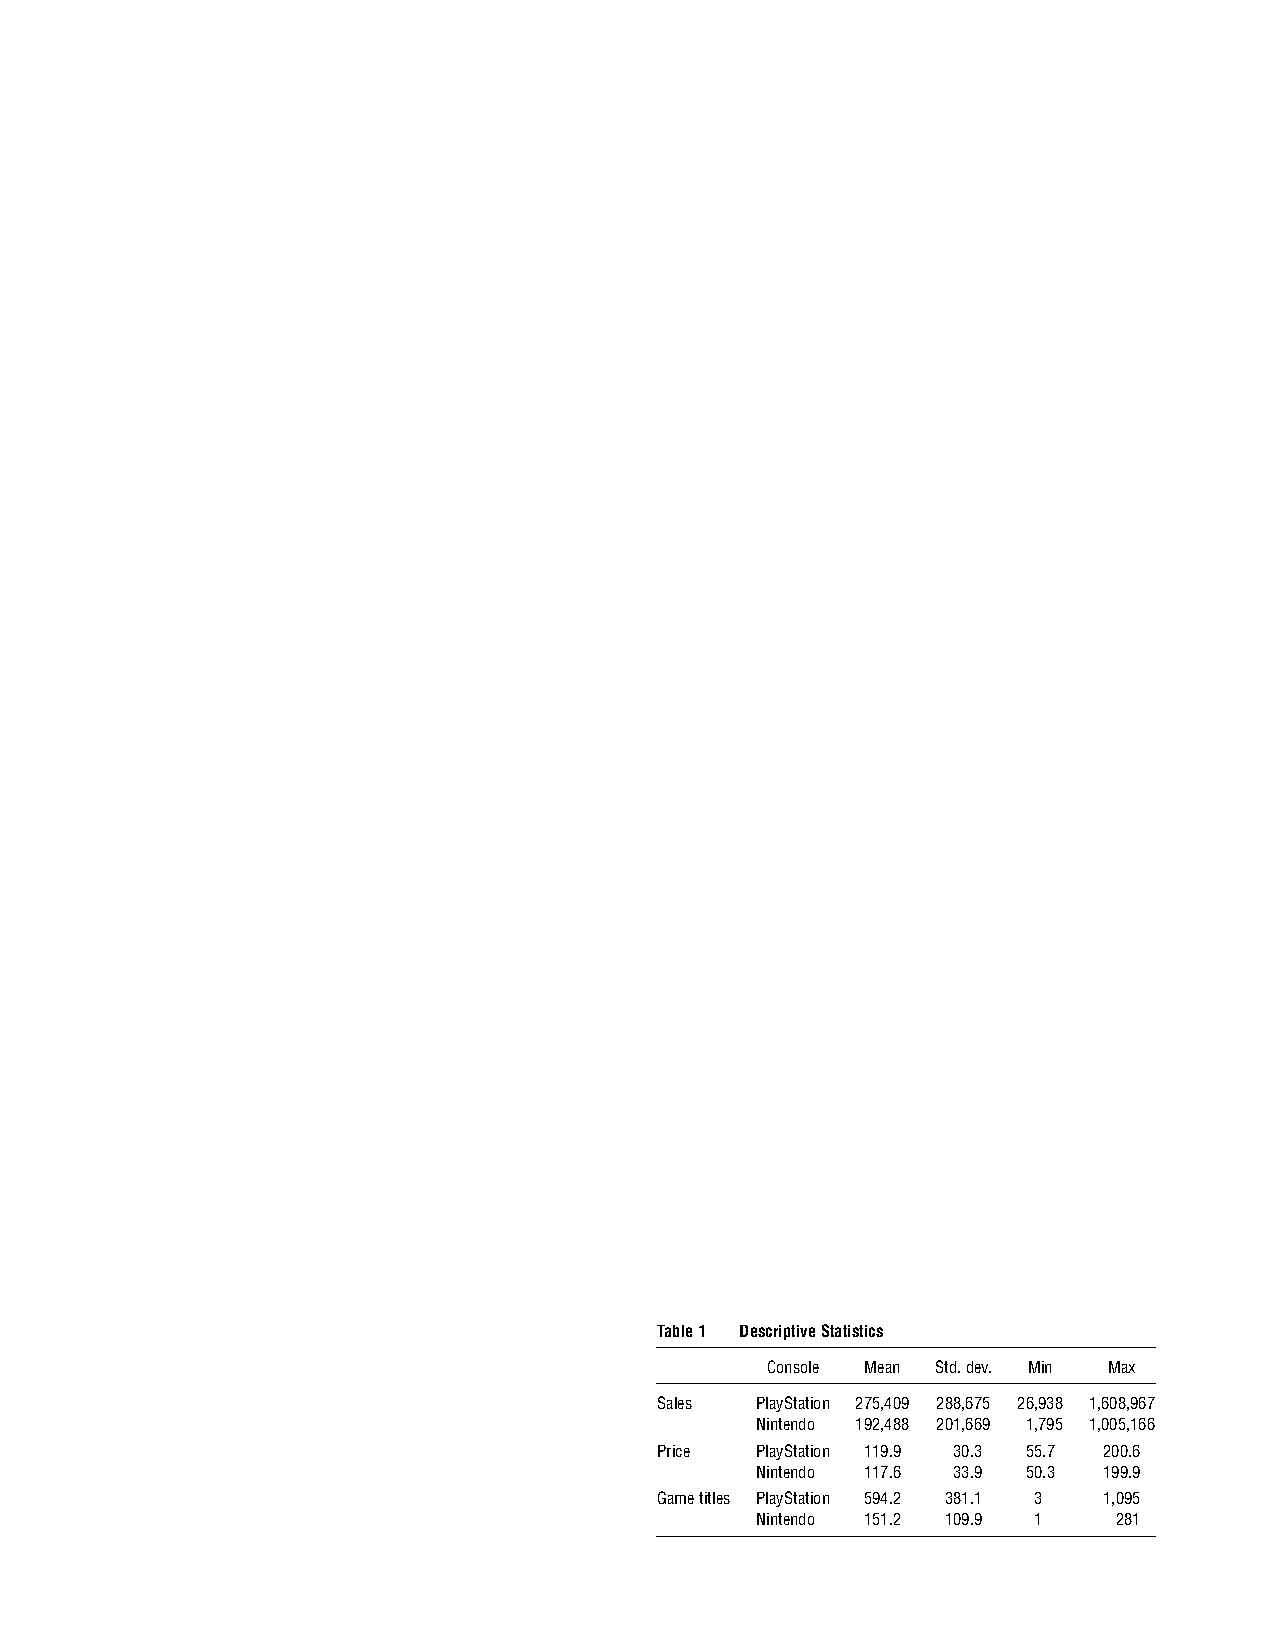
\includegraphics[scale=0.5]{resources/dube-table1}\\
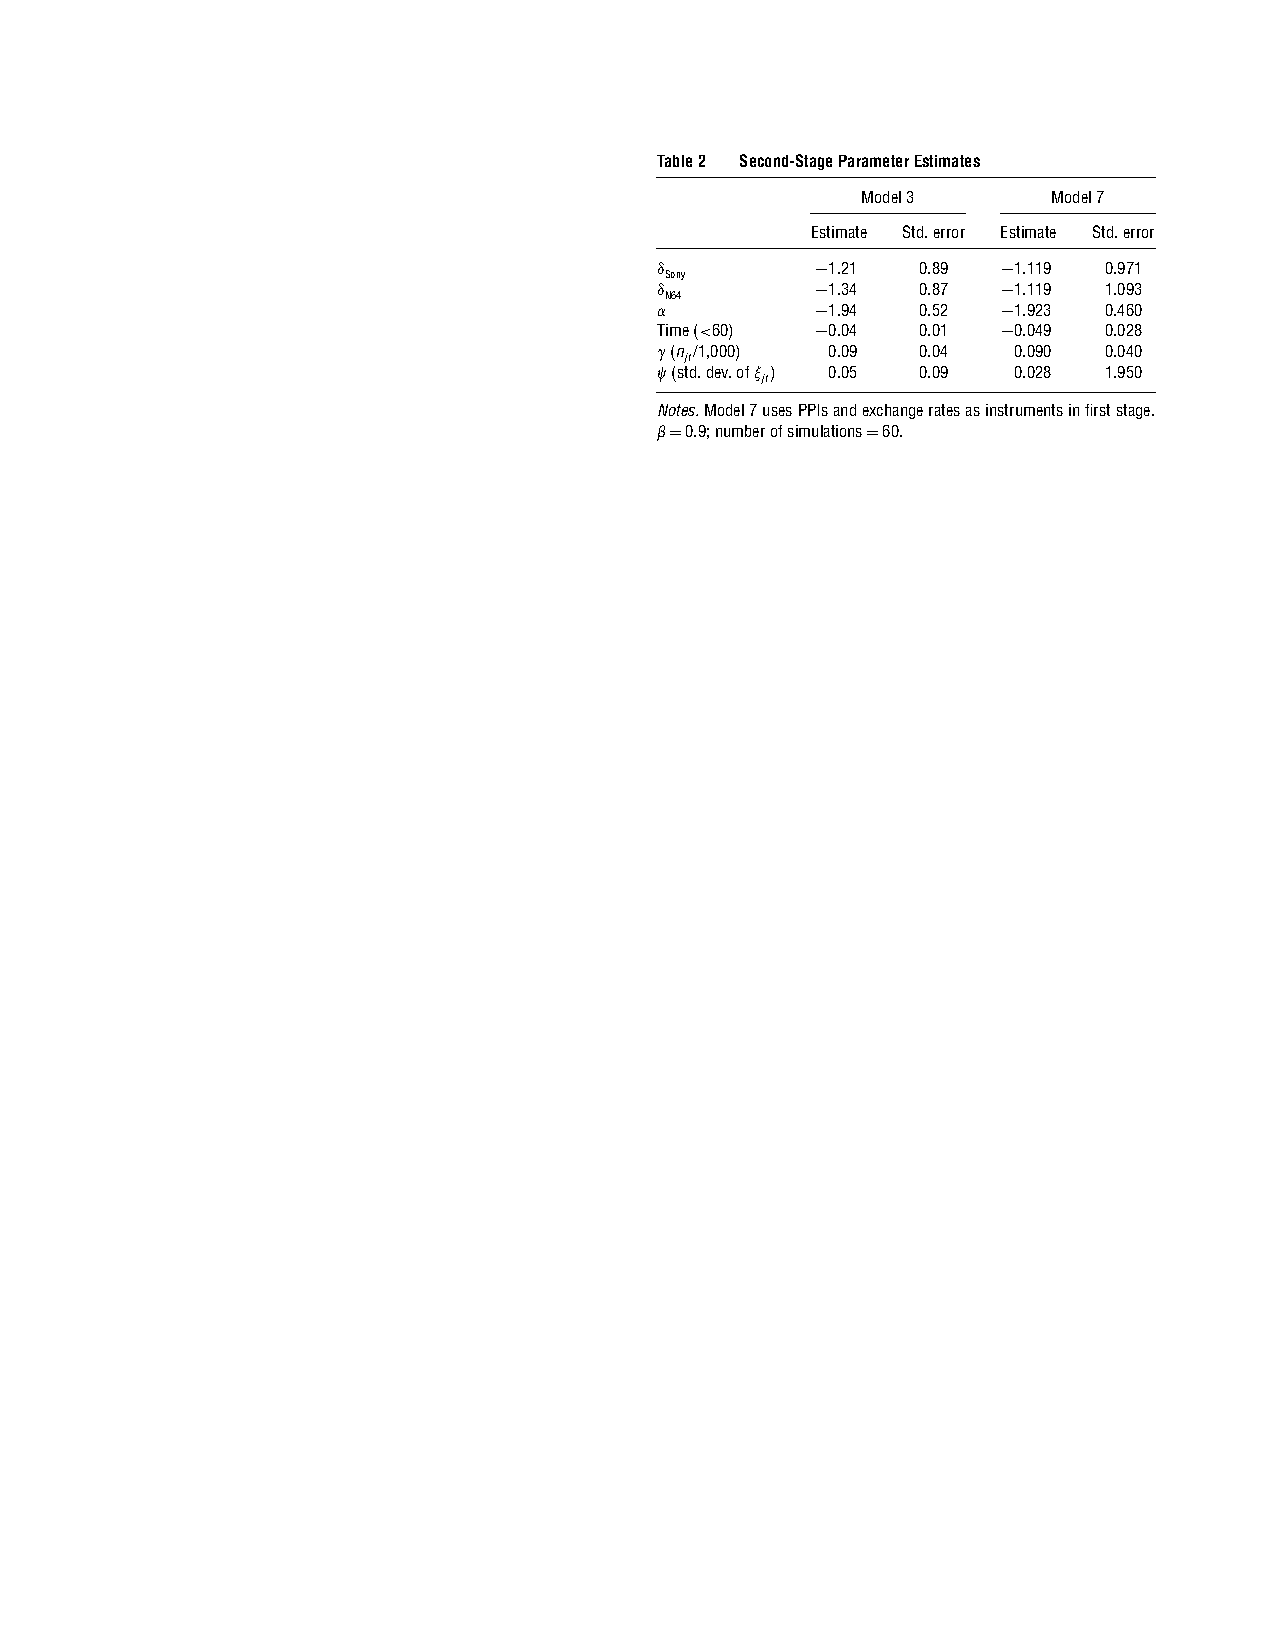
\includegraphics[scale=0.5]{resources/dube-table2}
\end{center}
\end{frame}

\begin{frame}{Counterfactual}
Suppose we got rid of network effects, how much lower would the concentration of the market be?
\end{frame}

\begin{frame}{Results}
\begin{center}
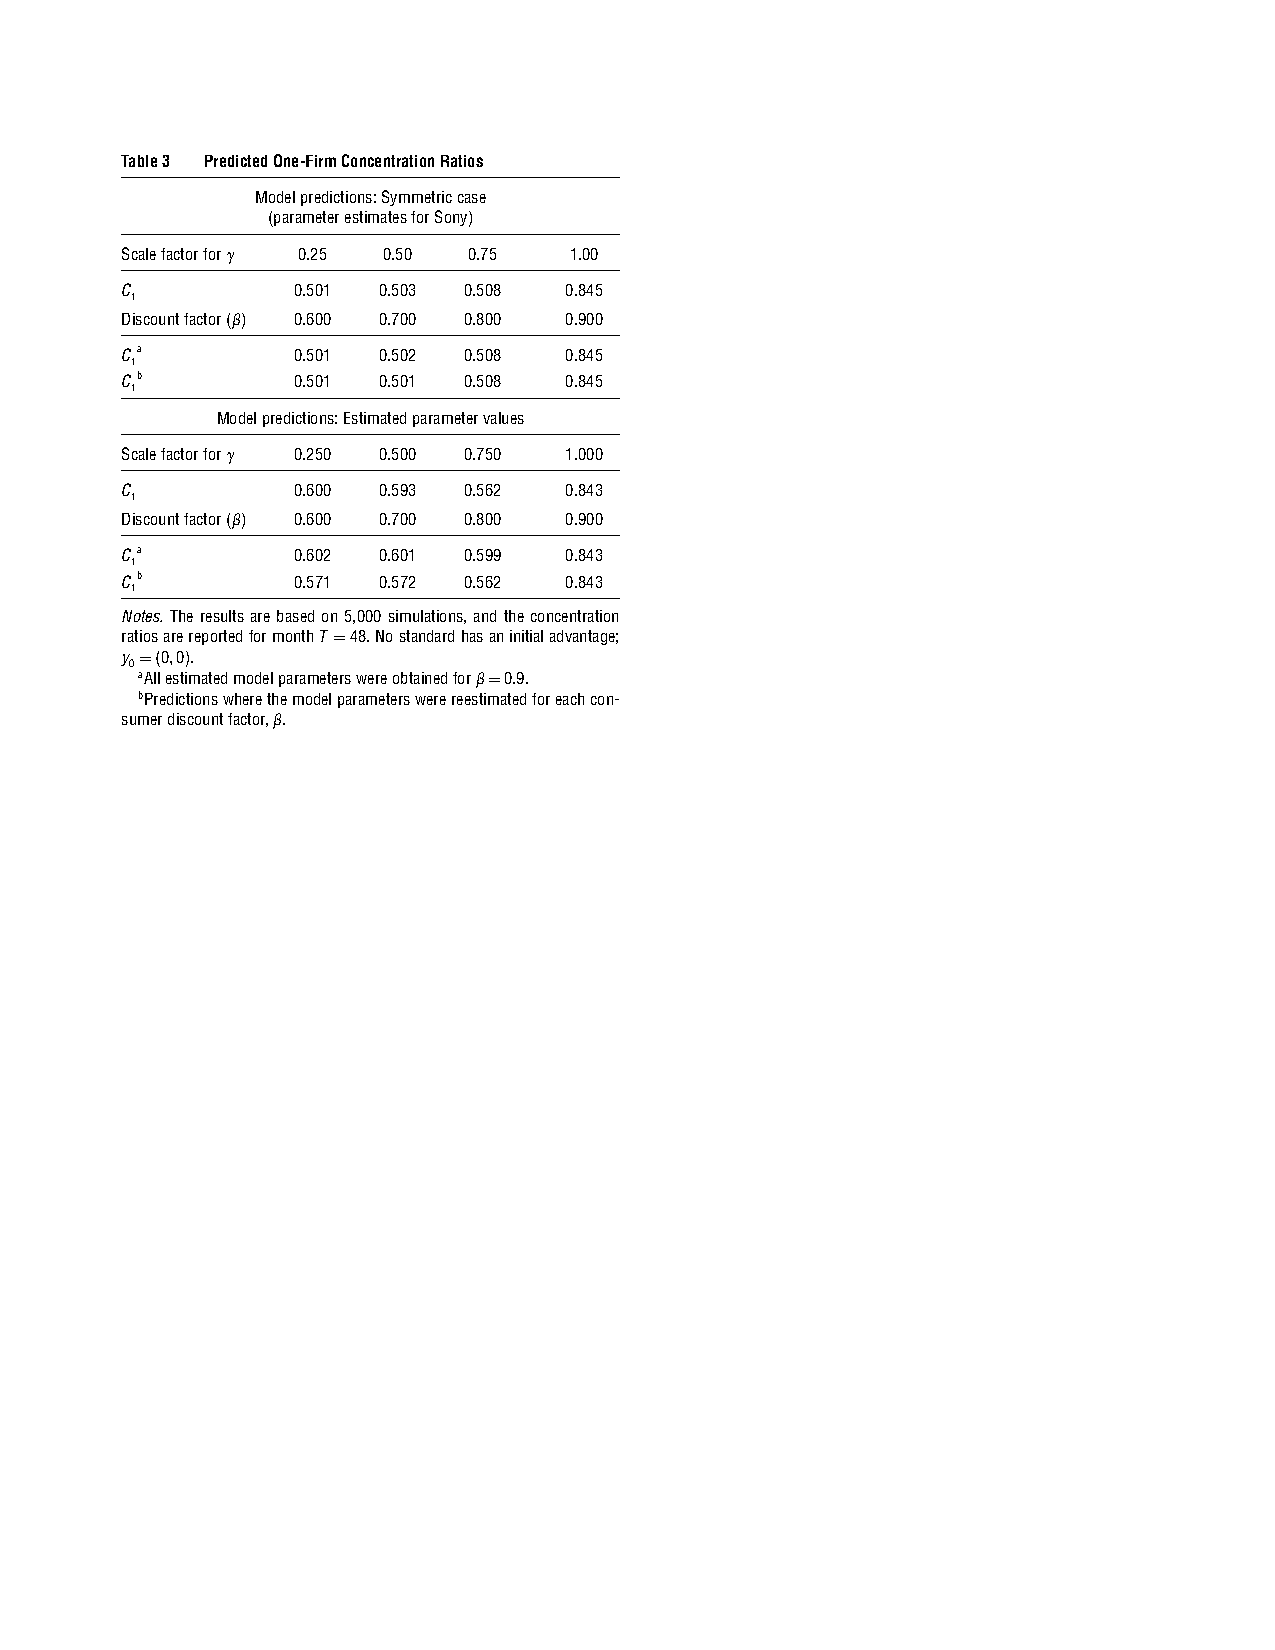
\includegraphics[scale=0.65]{resources/dube-table3}
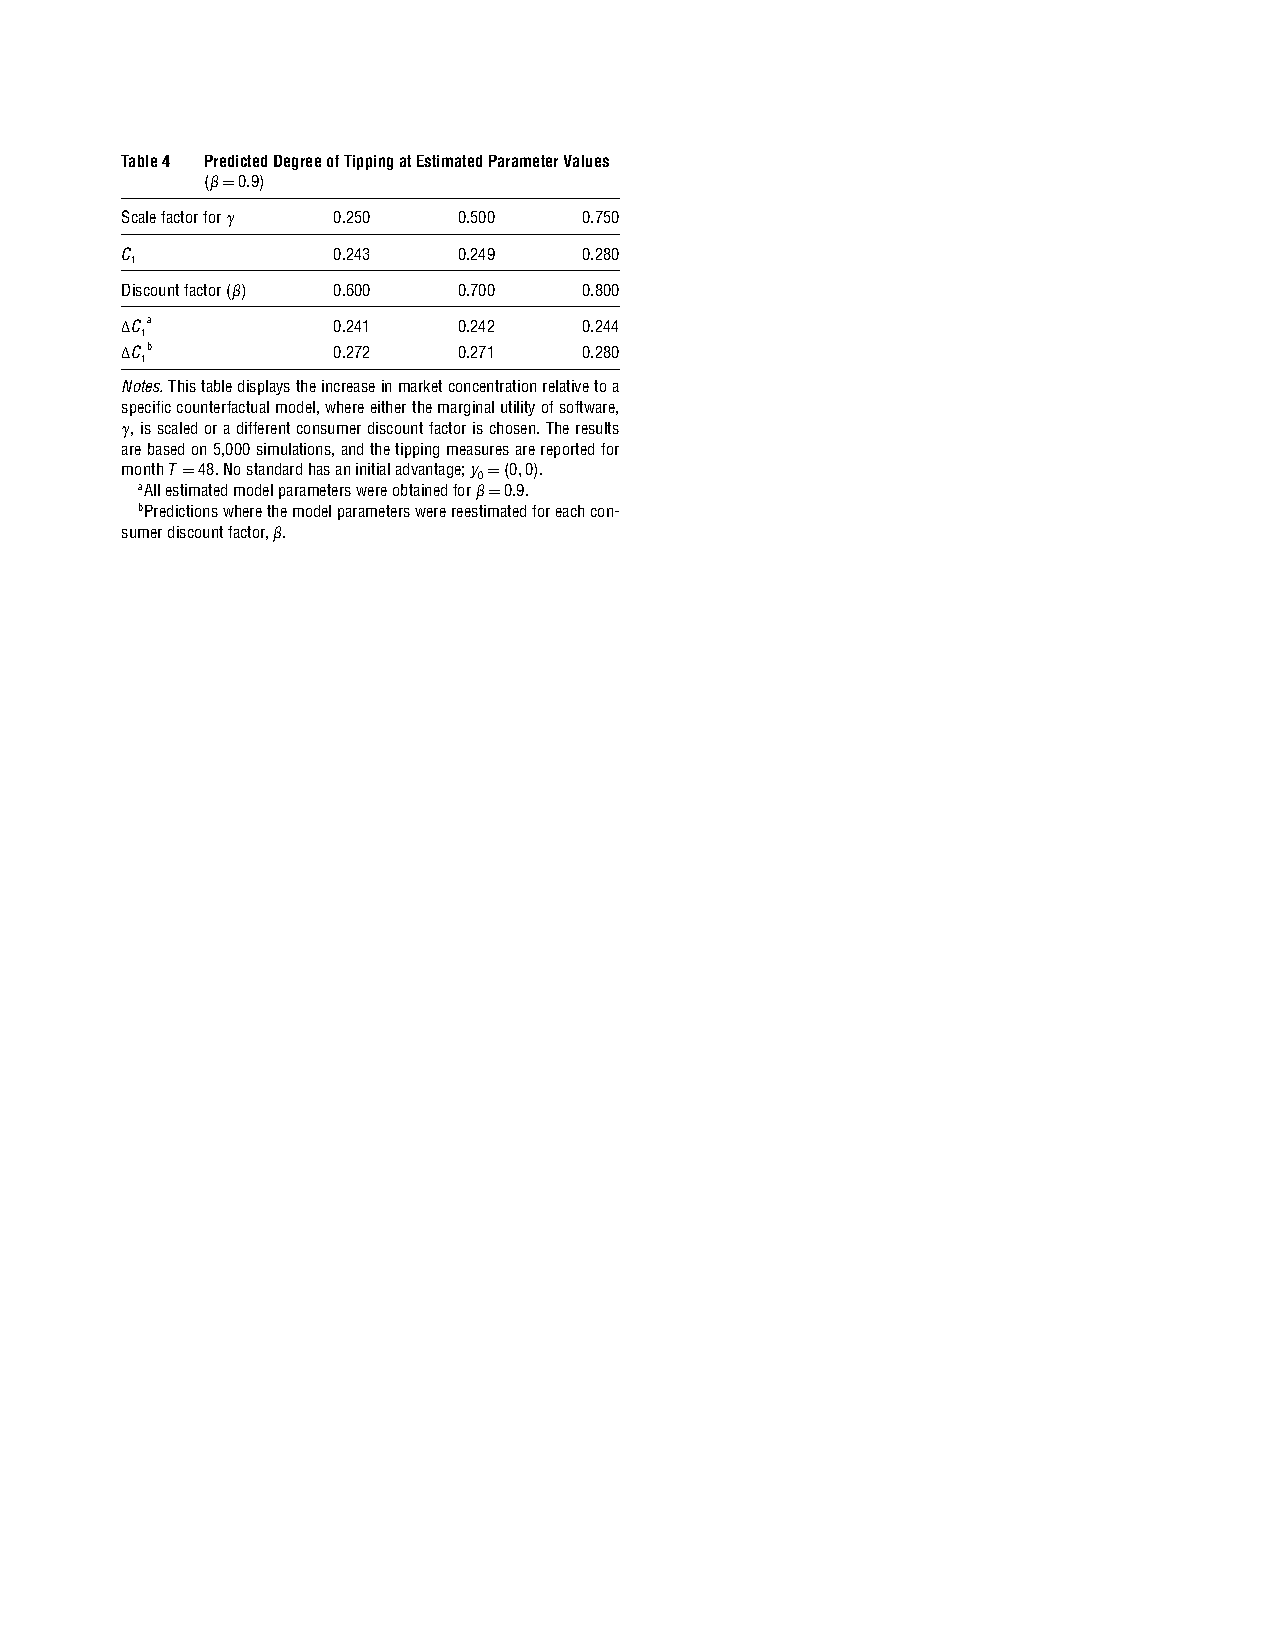
\includegraphics[scale=0.65]{resources/dube-table4}\\
\end{center}
\end{frame}

\begin{frame}{Results}
\begin{center}
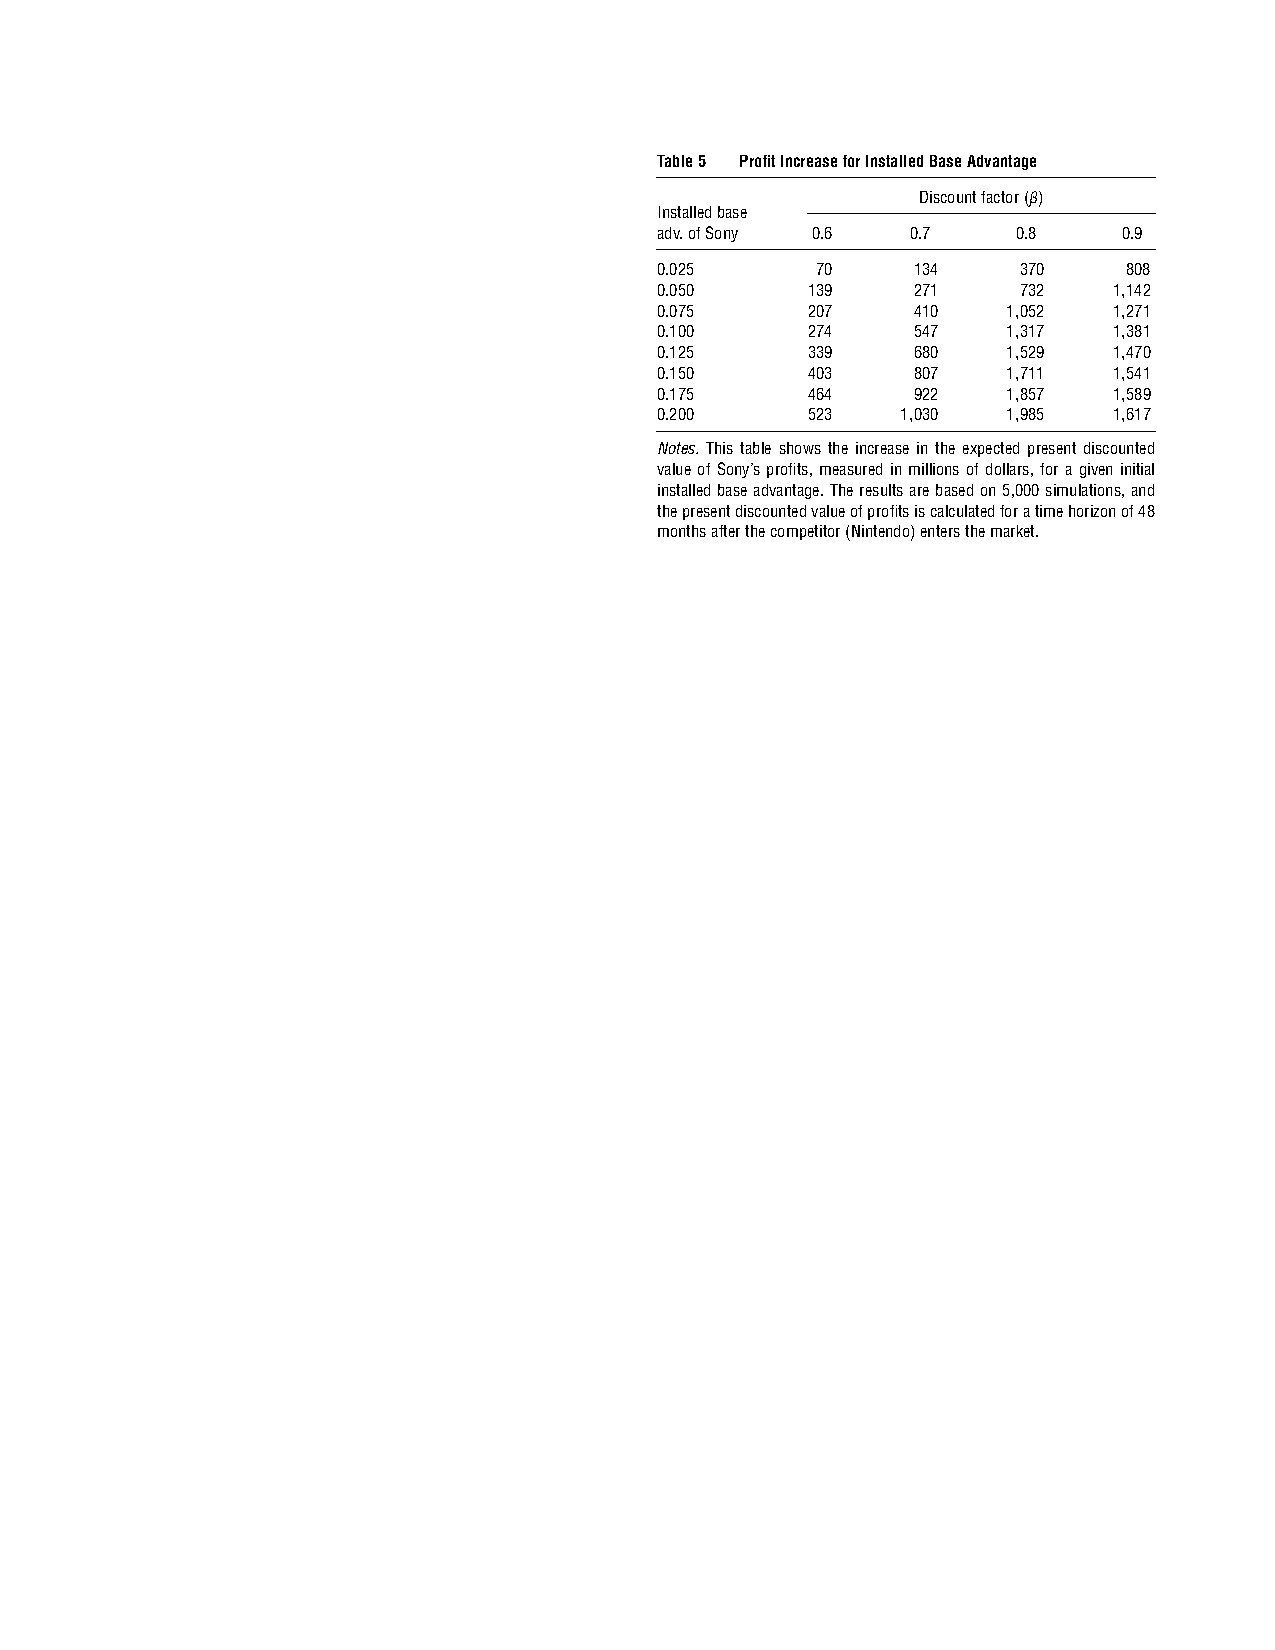
\includegraphics[scale=0.75]{resources/dube-table5}
\end{center}
\end{frame}


\end{document}













































